\chapter{Nguyên lý hoạt động}
\section{Cấu tạo}
Do Copilot là công cụ được tích hợp giữa tính năng tìm kiếm (search engines) và Chat GPT 4, nên ở trong chương 3 này
chúng ta sẽ tập trung vào nguyên lý hoạt động của Chat GPT. ChatGPT được cấu tạo bởi hai phần tử chính là Transformer model (mô hình biến đổi) và Language model (mô hình ngôn ngữ).
\subsection{Transformer model}
Transformer model là một loại kiến trúc mạng lưới nơ-ron (neural network architecture)
được thiết kế để có thể tạo ra thông tin một cách liên tục. Transformer thực hiện quy trình xử lý input bằng encoder và sau đó decoder (sử dụng context được cung cấp bởi encoder) tạo ra các output tương ứng \cite{link_6}. Mô hình đơn giản của transformer model có thể minh họa như sau \cite{link_7}:
\begin{figure}[h]
    \centering
    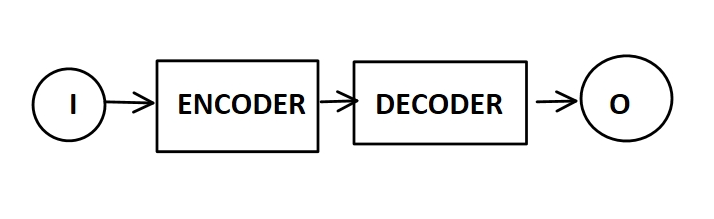
\includegraphics[width=0.8\textwidth]{transformer.png}
    \caption{Mô hình hoạt động của Transformer model}
\end{figure}
\subsection{Language model}
Language model (mô hình ngôn ngữ) là một mô hình được huấn luyện để dự đoán các từ tiếp theo trong một câu nhằm tạo ra các đoạn văn bản mạch lạc, logic và có ý nghĩa. Mô hình này có thể tự viết ra rất đa dạng các thể loại văn bản tùy theo mục đích của người sử dụng. Mô hình đơn giản của language model có thể minh họa như sau:
\begin{figure}[h]
    \centering
    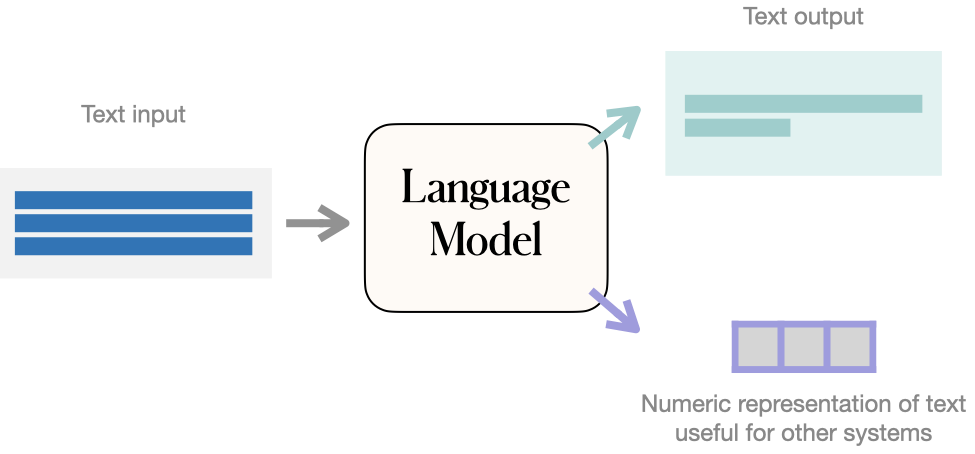
\includegraphics[width=0.8\textwidth]{Cohere-Language-Model.png}
    \caption{Mô hình hoạt động của Language model}
\end{figure}
\section{Nguyên lý hoạt động}
Giả sử khi người sử dụng nhập vào một câu chưa hoàn chỉnh chẳng hạn như "Quantum mechanics is", mô hình sẽ tìm kiếm và dự đoán các từ có khả năng xuất hiện tiếp theo trong output sao cho phù hợp với ngữ cảnh của cả câu văn rồi
thực hiện sắp xếp khả năng xuất hiện của các từ theo xác suất từ cao đến thấp: \cite{link_8}
\begin{itemize}
    \item Quantum mechanics is a...(4.5\%)
    \item Quantum mechanics is based...(3.8\%)
    \item Quantum mechanics is described...(3.2\%)
    \item Quantum mechanics is many...(0.7\%)
\end{itemize}
Sau đó mô hình sẽ lựa chọn giữa các từ "a", "based", "described", "many" để thêm vào trong câu trả lời. Quá trình này sẽ được lặp
lại liên tục cho đến khi câu trả lời được hoàn tất. Thế nhưng không nhất thiết lúc nào mô hình cũng lựa chọn từ với xác suất xuất hiện cao nhất, điều này nhằm tăng thêm tính ngẫu nhiên và sáng tạo của các câu trả lời do AI tạo ra.
Chẳng hạn như thay vì chọn "a" với xác suất cao nhất, AI hoàn toàn có thể lựa chọn "based" để hoàn thành một câu như sau:
\\"Quantum mechanics is based on a set of fundamental principles of morden physics."
\\Qua đây ta có thể thấy rằng AI có thể tạo ra rất nhiều câu trả lời phong phú nhưng vẫn phù hợp với ngữ cảnh.
\section{Quy trình huấn luyện AI}
Để có thể đưa ra các câu trả lời hoàn chỉnh và giống với ngôn ngữ "người" nhất, AI phải trải qua 3 giai đoạn huấn luyện (training) gồm:
\subsection{Giai đoạn 1}
Trong giai đoạn 1, người huấn luyện sẽ đóng cả hai vai trò là người sử dụng (user) và một chatbot lý tưởng (ideal chatbot) và tạo ra các cuộc hội thoại. Thông qua quá trình này, AI có thể học được từ các điểm tương đồng giữa các cuộc hội thoại để từ đó có thể tạo ra các câu trả lời 
gần giống với ngôn ngữ "người" nhất.
\subsection{Giai đoạn 2}
Trong giai đoạn 2, nhà phát triển sẽ "dạy" AI cách để đánh giá hay xếp hạng các output. Chẳng hạn như đối với yêu cầu "Describe an atom.", có 3 output tương ứng và được người huấn luyện xếp hạng như sau:\cite{link_8}
\begin{enumerate}
    \item It's the smallest part of a substance made of protons, electrons and neutrons.
    \item It's a basic chemical element.
    \item It's a ticketing service.
\end{enumerate}
AI sẽ nhận thứ tự sắp xếp theo độ chính xác 1>2>3 và sẽ đưa ra câu trả lời thứ 1 khi được yêu cầu trả lời.
\subsection{Giai đoạn 3}
Ở giai đoạn này, AI có thể tự học thông qua khả năng học tăng cường (reinforcement learning - RF) để có thể xử lý được các câu hỏi ở dạng "mở" như "Write a short story.", loại câu hỏi không có output rõ ràng.
AI đã có thể xử lý một lượng khổng lồ các bài báo, bài viết,... của con người trên internet để tổng hợp, phân tích và tìm các điểm chung giữa chúng để có thể tạo ra câu trả lời hợp lý nhất. Hiện nay, các AI mạnh như ChatGPT còn có khả năng học tăng cường từ các phản hồi của người dùng (reinforcement learning from human feedbacks - RLHF),
điều này càng làm tăng sức mạnh của công cụ trí tuệ nhân tạo.
